\chapter{Architectural Views} \label{ArchitecturalViews}

\section{Functional View}

\subsection{Stakeholders’ Uses of This View}

The Functional View defines the system’s runtime functional elements—their responsibilities, interfaces, and primary interactions—and shows how these collaborate to realize KSO’s required capabilities.

This view addresses the concerns listed in Table 17-2 of Rozanski \& Woods—functional capabilities, external interfaces, internal structure, and overall design philosophy—and serves as a cornerstone of the architectural description. Different stakeholder classes use it as follows:

\begin{itemize}
    \item \textbf{Marine Ecologists (Users)}\\
    Verify that the system provides the analytic and export functions they need (e.g., species-count dashboards, spatial-distribution queries).\\
    Understand how data flows from ingestion through model inference to visualization, so they can plan their research workflows against the system’s capabilities.

    \item \textbf{Citizen Scientists (Users)}\\
    Comprehend the clip-classification and annotation pipelines—how their inputs (clip labels, bounding boxes) propagate through the consensus aggregator to the database.\\
    See which external interfaces (web-UI endpoints, tutorial workflows) they will interact with during annotation tasks.

    \item \textbf{ML Engineers \& Developers}\\
    Inspect component interactions (e.g., video-splitter $\rightarrow$ preprocessing service $\rightarrow$ training orchestrator $\rightarrow$ inference API) to validate separation of concerns, loose coupling, and latency-sensitive paths.\\
    Use sequence and activity diagrams derived from this view to plan unit and integration tests, and to guide implementation of connector protocols (RPC, messaging, REST).

    \item \textbf{System Administrators}\\
    Understand which functional elements (e.g., metadata service, model-serving endpoint, consensus engine) must be deployed on which hosts or containers.\\
    Plan monitoring and failure-recovery strategies by tracing runtime paths between elements and identifying critical connectors (message queues, API gateways).

    \item \textbf{Project Sponsors / Acquirers}\\
    Assess that all high-level functional requirements (ingestion, annotation, model inference, visualization) are covered by well-defined elements and interfaces.\\
    Evaluate architectural flexibility—how easily new functions (e.g., support for additional taxa) could be slotted into the existing component graph without wholesale redesign.

    \item \textbf{Testers}\\
    Derive test scenarios by walking through common use cases (e.g., ``submit a clip $\rightarrow$ receive bounding-box review'') against the interaction paths shown in component and sequence diagrams.\\
    Identify boundary points for black-box testing (REST endpoints, messaging topics) and white-box tests (component method contracts, error-handling flows).
\end{itemize}

By tailoring the level of abstraction and notation (UML component diagrams, sequence diagrams, or simplified ``boxes-and-lines'' sketches) to each group’s background, the Functional View becomes an effective communication tool for both technical and non-technical stakeholders.

\subsection{Component Diagram}
We can see that Figure~\ref{fig:component-diagram} shows us the high-level component structure of the Koster Seafloor Observatory (KSO), with all relationships indicated.

\begin{figure}[ht]
  \centering
  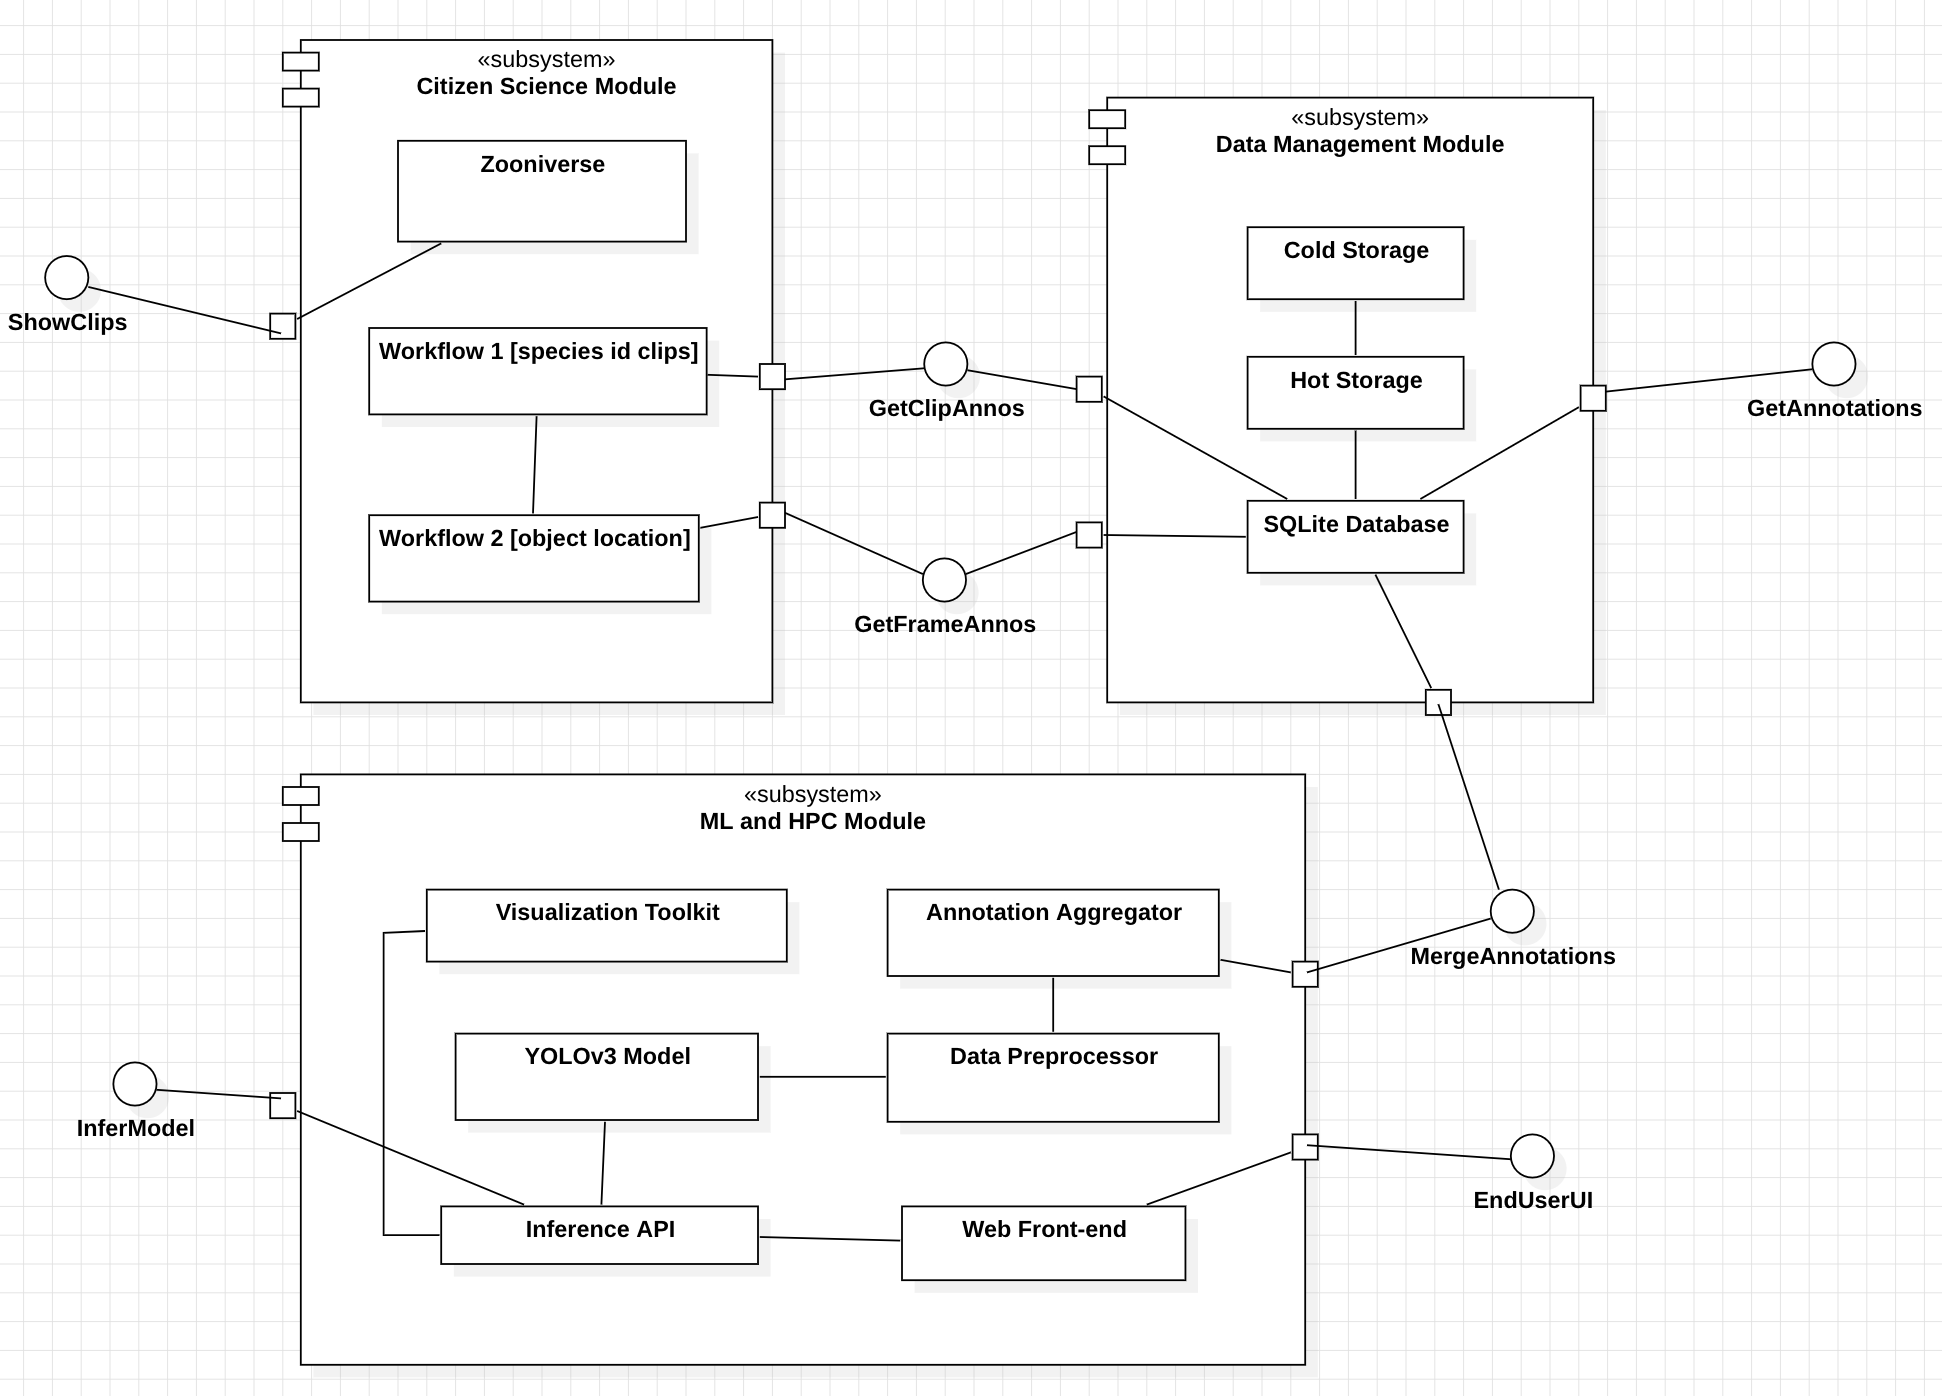
\includegraphics[width=\textwidth]{Figures/ComponentDiagram.png}
  \caption{Component Diagram of KSO}
  \label{fig:component-diagram}
\end{figure}

\paragraph{Component Descriptions:}
\begin{itemize}
  \item \textbf{Data Management Module}
    \begin{itemize}
      \item \textbf{Cold Storage} (\verb|<<component>>|): long‐term archive of raw subsea video files.
      \item \textbf{Hot Storage} (\verb|<<component>>|): HPC server holding the active working set of clips.
      \item \textbf{SQLite Database} (\verb|<<component>>|): stores metadata, clip/frame records, and annotation results.
    \end{itemize}

  \item \textbf{Citizen Science Module}
    \begin{itemize}
      \item \textbf{Zooniverse Project Site} (\verb|<<component>>|): web portal exposing the two annotation workflows.
      \item \textbf{Workflow 1: Species Identification} (\verb|<<component>>|): presents 10 s clips for volunteer species labelling.
      \item \textbf{Workflow 2: Object Localization} (\verb|<<component>>|): allows volunteers to draw bounding boxes on frames.
    \end{itemize}

  \item \textbf{Machine Learning \& HPC Module}
    \begin{itemize}
      \item \textbf{Annotation Aggregator} (\verb|<<component>>|): merges citizen annotations based on agreement thresholds.
      \item \textbf{Data Preprocessor} (\verb|<<component>>|): performs frame‐level tracking, augmentation, and normalization.
      \item \textbf{YOLOv3 Model} (\verb|<<component>>|): trains and tests detection on preprocessed frames.
      \item \textbf{Inference API} (\verb|<<component>>|, FastAPI): exposes prediction endpoints for the trained model.
      \item \textbf{Web Front‐end} (\verb|<<component>>|, Streamlit): researcher‐facing UI for uploading footage and tuning thresholds.
      \item \textbf{Visualization Toolkit} (\verb|<<component>>|): generates spatial and temporal distribution maps.
    \end{itemize}
\end{itemize}

\paragraph{Interfaces (\texttt{<<provides>>}/\texttt{<<requires>>})}
\begin{itemize}
  \item \texttt{Cold Storage} \texttt{<<provides>>} raw video clips to \texttt{Hot Storage}.
  \item \texttt{Hot Storage} \texttt{<<provides>>} clip metadata to \texttt{SQLite Database}.
  \item \texttt{SQLite Database} \texttt{<<provides>>} clips and metadata to \texttt{Workflow 1} and \texttt{Workflow 2}.
  \item \texttt{Workflow 1, Workflow 2} \texttt{<<provides>>} citizen annotations back to \texttt{SQLite Database}.
  \item \texttt{SQLite Database} \texttt{<<provides>>} aggregated frames to \texttt{Annotation Aggregator}.
  \item \texttt{Annotation Aggregator} \texttt{<<provides>>} cleaned, tracked frames to \texttt{Data Preprocessor}.
  \item \texttt{Data Preprocessor} \texttt{<<provides>>} training/test datasets to \texttt{YOLOv3 Model}.
  \item \texttt{YOLOv3 Model} \texttt{<<provides>>} inference service to \texttt{Inference API}.
  \item \texttt{Inference API} \texttt{<<provides>>} prediction endpoints consumed by \texttt{Web Front‐end} and \texttt{Visualization Toolkit}.
\end{itemize}

\subsection{Internal Interfaces}

\begin{figure}[H]
    \centering
    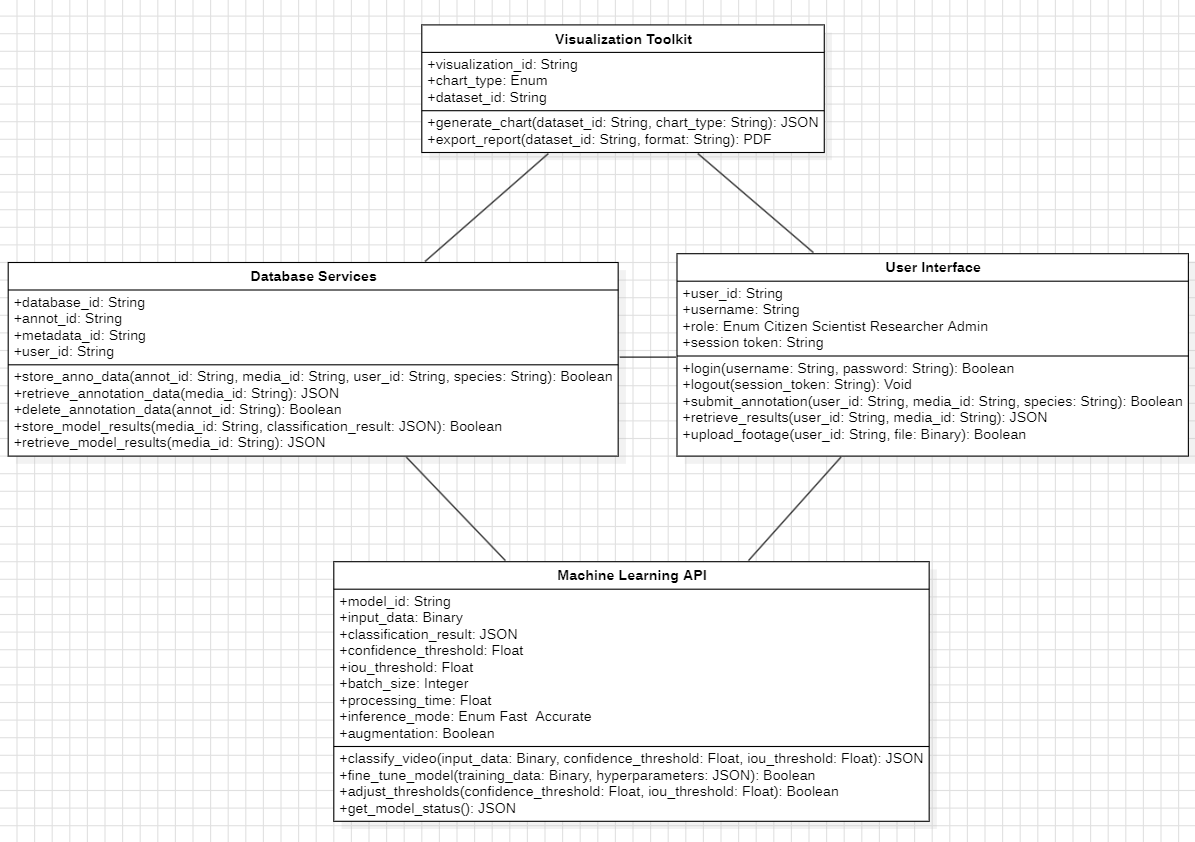
\includegraphics[width=1 \textwidth]{Figures/InternalInterface.png}
    \caption{Internal Interfaces Class Diagram \label{Fig:Internal Interfaces}}
\end{figure}


\textbf{User Interface}
Serving the User Interface’s needs, this interface provides authentication (login/logout), annotation CRUD, result retrieval, and raw footage upload operations against the core Database Services. All methods accept JSON over REST and validate session tokens, enabling the front-end (web or Streamlit) to securely manage user sessions, persist annotations, fetch past results for display, and store newly uploaded videos without exposing database details to the client.

\textbf{Database Service Interface}
This interface abstracts the orchestration between Database Services and underlying Storage Services by offering methods to store, retrieve, and delete media files; it also supports moving files between hot and cold storage tiers. Calls carry binary payloads alongside metadata in JSON and specify the desired storage type, allowing KSO to optimize cost and performance by automatically archiving infrequently accessed footage while keeping active datasets on faster disks.

\textbf{Machine Learning API Interface}
Acting as the bridge between Database Services and the Machine Learning API, this interface lets the database layer request video classification (with configurable confidence and IOU thresholds), store the JSON-formatted detection results, retrieve past model outputs, adjust inference parameters on the fly, and query model training status. All operations use REST+JSON, making it easy for the database to orchestrate inference workflows and record machine-generated annotations alongside citizen-science data.

\textbf{Visualization Toolkit Interface}
This interface connects Database Services to the Visualization Toolkit by exposing operations to generate chart specifications (bar, line, heatmap, etc.) in JSON and export fully rendered reports in binary formats (PDF or HTML). By decoupling visualization concerns, KSO can produce interactive dashboards and print-ready summaries without embedding plotting logic in the core data services, ensuring a clean separation between data management and presentation layers.

\newpage
\subsection{Interaction Patterns}

\begin{figure}[H]
    \centering
    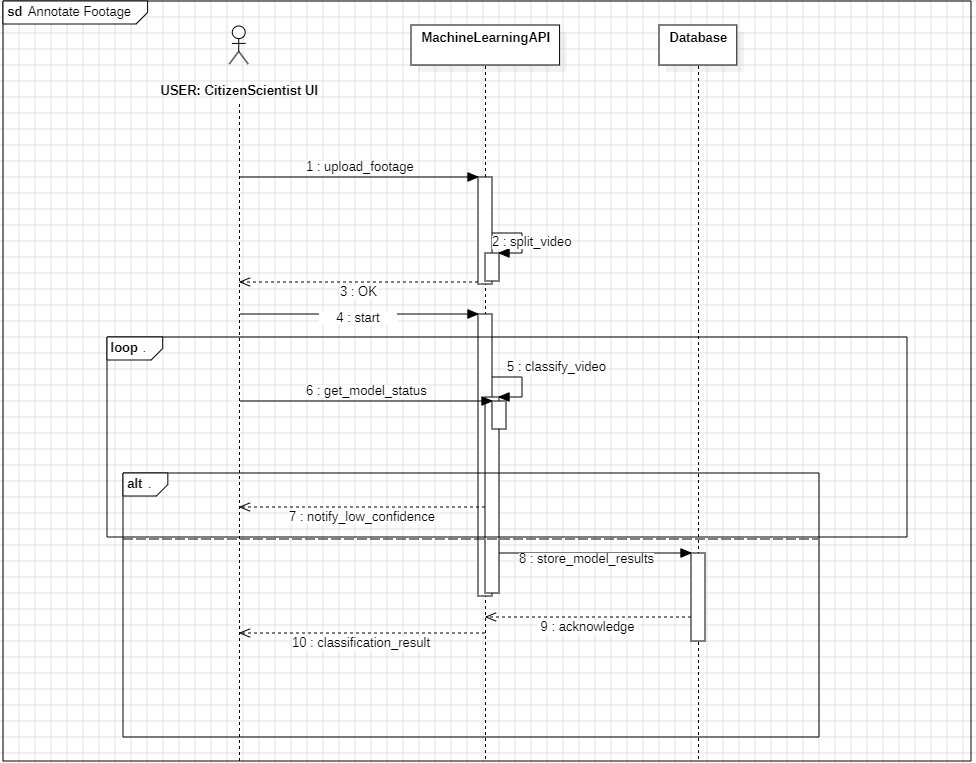
\includegraphics[width=1 \textwidth]{Figures/SequenceDiagram1.png}
    \caption{Sequence Diagram for Annotate Footage\label{Fig:Sequence Diagram}}
\end{figure}


\begin{figure}[H]
    \centering
    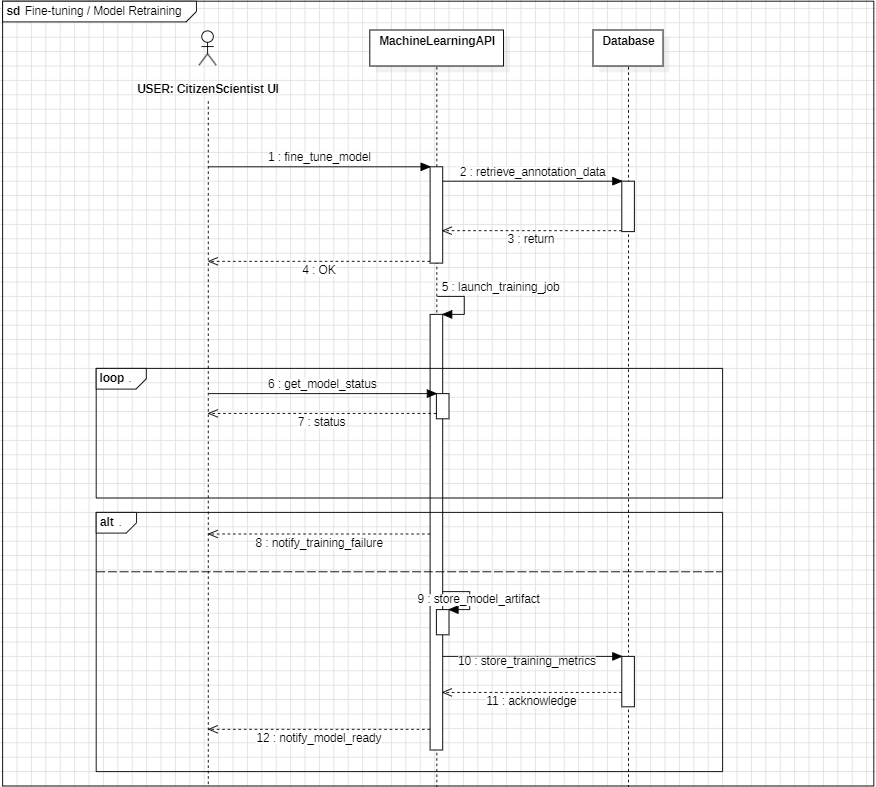
\includegraphics[width=1 \textwidth]{Figures/SequenceDiagram2.png}
    \caption{Sequence Diagram for Fine Tuning ML Models\label{Fig:Sequence Diagram }}
\end{figure}

\begin{figure}[H]
    \centering
    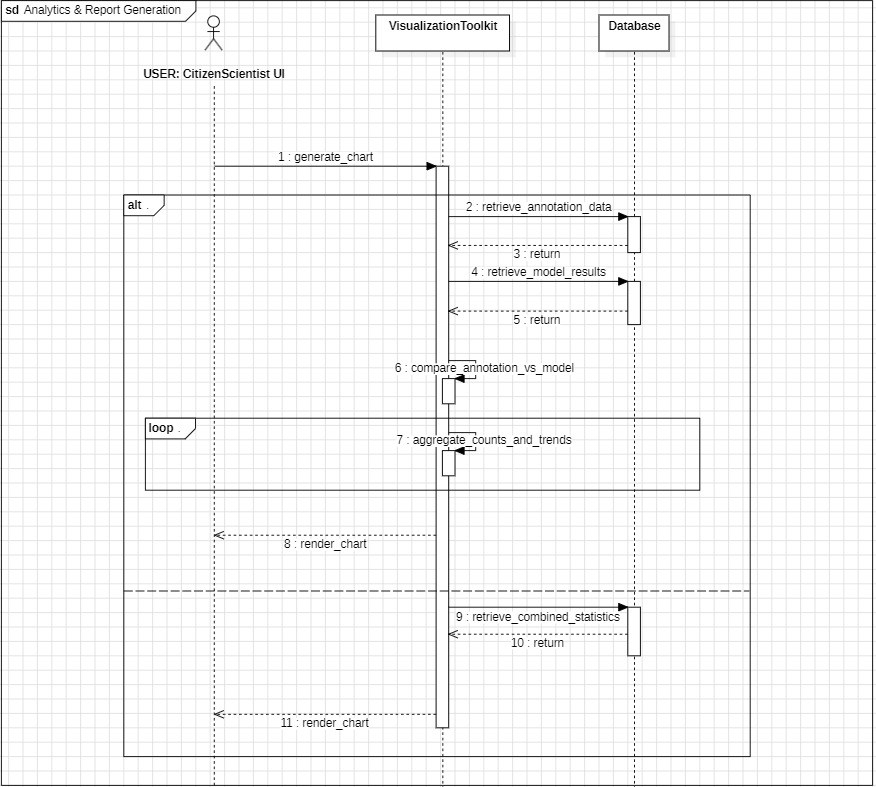
\includegraphics[width=1 \textwidth]{Figures/SequenceDiagram3.png}
    \caption{Sequence Diagram for Analytics and Report Generation\label{Fig:Sequence Diagram }}
\end{figure}

\subsection{External Interfaces}
\begin{figure}[H]
    \centering
    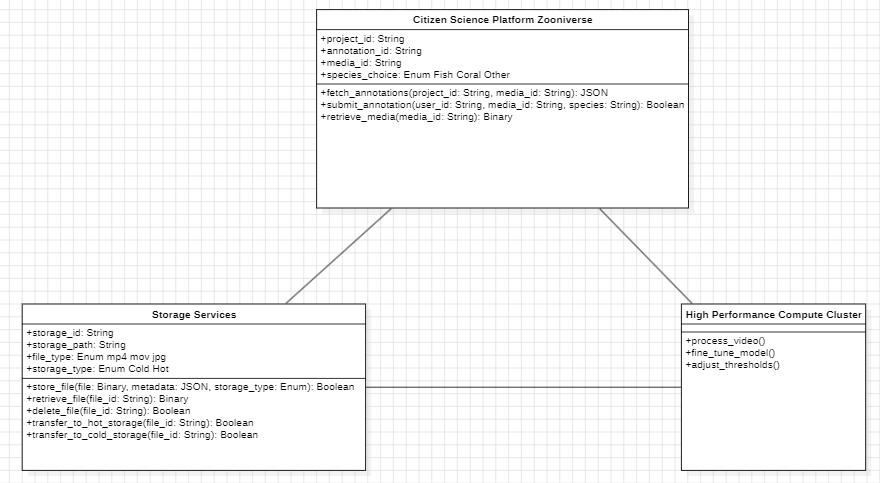
\includegraphics[width=1 \textwidth]{Figures/ExternalInterface.png}
    \caption{External Interfaces Class Diagram \label{Fig:External Interfaces}}
\end{figure}

\textbf{Citizen Science Platform Interface}
This interface encapsulates all interactions with the Zooniverse citizen-science platform: it fetches project and workflow definitions (so that KSO knows which species and annotation tasks to present), uploads 10-second video clips for volunteer classification, submits individual user annotations back to Zooniverse, and retrieves both raw and aggregated annotation results. All operations use REST over HTTPS with JSON payloads and OAuth2 authentication, ensuring that KSO can seamlessly offload clip distribution and annotation collection to an established crowdsourcing service.

\textbf{Storage Services}
This interface handles the push and query of metadata records to the Swedish National Data Archive using Darwin Core standards. It allows KSO to deposit or update metadata (e.g., location, date, camera settings) for each uploaded movie, perform spatial/temporal/keyword searches against archived datasets, and list all datasets associated with a given project. Communication occurs over HTTP(S) using either JSON or XML (CSW/OAI-PMH style) with API-Key or client-certificate authentication, guaranteeing that KSO’s scientific outputs remain interoperable with national biodiversity data infrastructures.

\textbf{HPC Compute Cluster Interface}
This interface manages submission and monitoring of heavy compute jobs—such as ML training runs or batch inference—to an external high-performance computing cluster. KSO submits a JSON-encoded job configuration (container image, dataset locations, hyperparameters) and receives back a jobId; it can then poll that ID for status updates (“PENDING”, “RUNNING”, “DONE”, “FAILED”) and, upon completion, fetch the resulting model weights or inference outputs as binary artifacts. Transport may use a REST gateway or SSH/SFTP, ensuring that resource-intensive tasks scale without overloading the core KSO service.

\subsection{Interaction scenarios}

\begin{figure}[H]
  \centering
  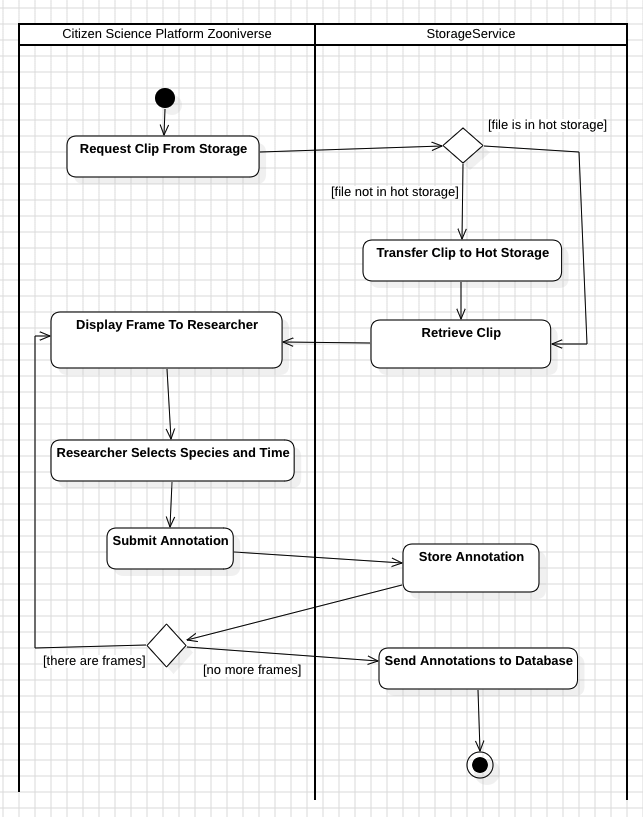
\includegraphics[width=1 \textwidth]{Figures/ActivityDiagram1.png}
  \caption{Activity Diagram for Annotate Footage\label{Fig:Activity Diagram 1}}
\end{figure}

\begin{figure}[H]
  \centering
  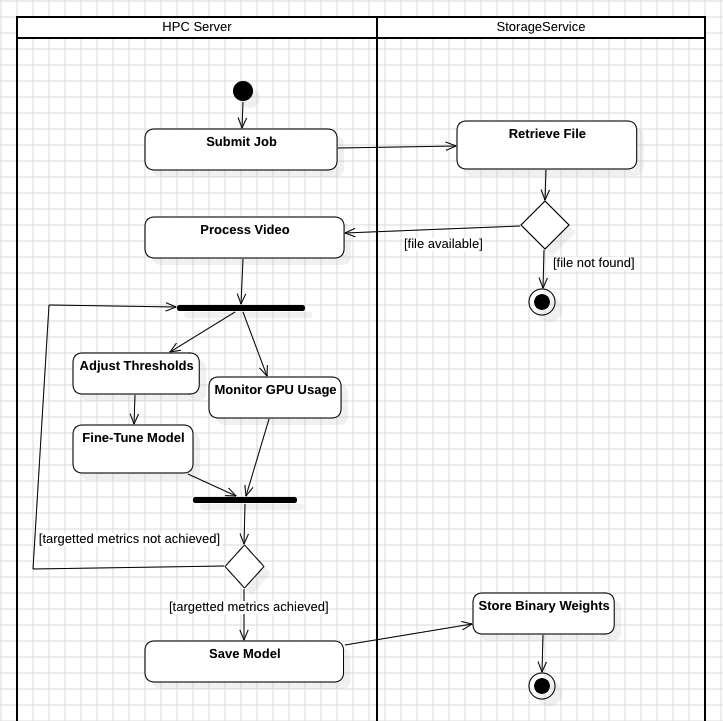
\includegraphics[width=1 \textwidth]{Figures/ActivityDiagram2.png}
  \caption{Activity Diagram for Fine Tuning ML Models\label{Fig:Activity Diagram 1}}
\end{figure}

\newpage
\section{Information View}

\subsection{Stakeholders’ Uses of This View}
The Information View exposes the structure and operations on the key persistent “objects” in KSO.  
Its primary consumers are:  
\begin{itemize}
  \item \textbf{Database Administrators (DBAs)} – to understand the schema, relationships, and lifecycle of each table/class.  
  \item \textbf{Backend Developers} – to see which methods they must implement in DAOs or repositories, and how entities relate.  
  \item \textbf{System Integrators} – to discover which operations exist for creating, querying, and linking domain data (e.g.\ projects, movies, annotations).  
  \item \textbf{QA/Test Engineers} – to identify boundary conditions (e.g.\ deleting a \texttt{Movie} must cascade or forbid if \texttt{Subject} exists).  
  \item \textbf{Product Owners / Analysts} – to verify that each real-world concept (e.g.\ “Species count in a clip”) is represented and manipulable in the API/DB.  
\end{itemize}

\subsection{Database Class Diagram}

\begin{figure}[H]
    \centering
    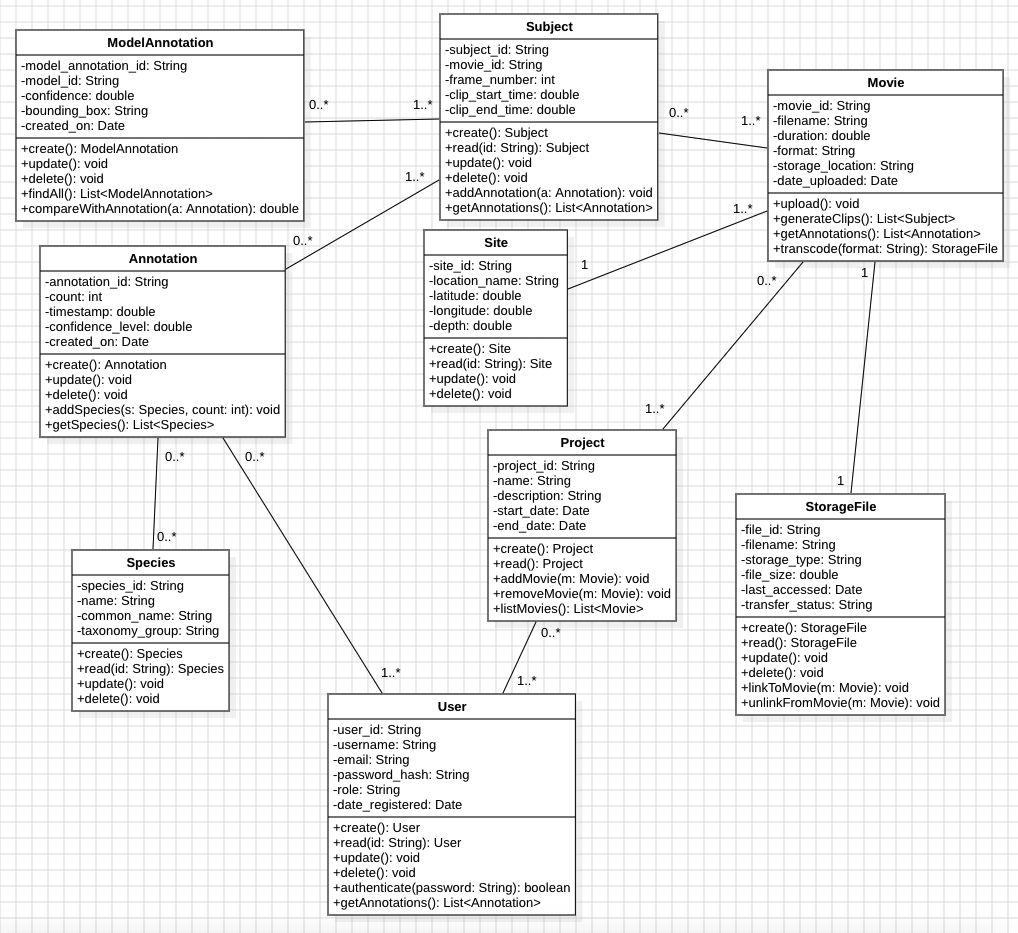
\includegraphics[width=1 \textwidth]{Figures/DatabaseClassDiagram.png}
    \caption{Database Class Diagram \label{Fig:Database Class Diagram}}
\end{figure}

Figure \ref{Fig:Database Class Diagram} models the eight core persistent entities of KSO and their navigations:
\begin{itemize}[noitemsep,leftmargin=*]
  \item \textbf{Project:}  
    Encapsulates a research campaign; owns zero or more \textbf{Movie} instances and provides methods to add, remove and list them.
  \item \textbf{Site:}  
    Represents a physical observation location; each Site hosts zero or more Movies.
  \item \textbf{Movie:}  
    Stores video metadata (filename, duration, format, upload date, storage URI).  
    Offers CRUD plus domain methods to generate \textbf{Subject} clips, retrieve human \textbf{Annotation}s, and transcode into new \textbf{StorageFile}s.
  \item \textbf{Subject:}  
    Defines a time-bounded segment of a Movie (frame number, start/end time).  
    Connects to both human (\textbf{Annotation}) and algorithmic (\textbf{ModelAnnotation}) annotations.
  \item \textbf{Annotation:}  
    Records a user-verified species count at a timestamp, links to one \textbf{User} and zero-to-many \textbf{Species} entries via its \texttt{addSpecies()} method.
  \item \textbf{ModelAnnotation:}  
    Captures machine-generated detections (model name, confidence, bounding box).  
    Can be compared to a human Annotation via \texttt{compareWithAnnotation()}.
  \item \textbf{StorageFile:}  
    Represents raw or processed file artifacts for a Movie (size, transfer status, last accessed).  
    Methods allow linking/unlinking to Movie records.
  \item \textbf{Species:}  
    Centralizes taxonomy data; referenced by Annotation to record counts per species.
  \item \textbf{User:}  
    Manages authentication/authorization and is the creator of zero or more Annotations.
\end{itemize}

\subsection{Operations on Data}
All classes support basic CRUD and finder methods, plus a few domain-specific navigations. Below we can list the key operations from the diagram:

\begin{longtable}{|l|l|}
    \caption{Operations on Data} \label{tab:operations-on-data} \\
    \hline
    Operation & Description \\
    \hline
    \endfirsthead
    \multicolumn{2}{c}%
    {{\bfseries Table \thetable\ continued from previous page}} \\
    \hline
    Operation & Description \\
    \hline
    \endhead
    
    \hline \multicolumn{2}{r}{{Continued on next page}} \\
    \endfoot
    
    \hline
    \endlastfoot
    
    CreateAccount & Create: User \\
                  & Read: - \\
                  & Update: - \\
                  & Delete: - \\
    \hline
    DeleteAccount & Create: - \\
                  & Read: - \\
                  & Update: - \\
                  & Delete: User \\
    \hline
    AddNewAnnotation & Create: Annotation \\
                     & Read: Subject \\
                     & Update: Subject (addAnnotation) \\
                     & Delete: - \\
    \hline
    DeleteAnnotation & Create: - \\
                     & Read: - \\
                     & Update: - \\
                     & Delete: Annotation \\
    \hline
    AddNewSpecies & Create: Species \\
                  & Read: Annotation \\
                  & Update: Annotation (addSpecies) \\
                  & Delete: - \\
    \hline
    DeleteSpecies & Create: - \\
                  & Read: - \\
                  & Update: - \\
                  & Delete: Species \\
    \hline
    UploadMovie & Create: - \\
                & Read: Movie \\
                & Update: Movie (upload, generateClips, transcode) \\
                & Delete: - \\
    \hline
    DeleteMovie & Create: - \\
                & Read: - \\
                & Update: - \\
                & Delete: Movie \\
    \hline
    CreateSite & Create: Site \\
               & Read: - \\
               & Update: - \\
               & Delete: - \\
    \hline
    DeleteSite & Create: - \\
               & Read: - \\
               & Update: - \\
               & Delete: Site \\
    \hline
    CreateProject & Create: Project \\
                 & Read: - \\
                 & Update: Project (addMovie, removeMovie) \\
                 & Delete: - \\
    \hline
    DeleteProject & Create: - \\
                 & Read: - \\
                 & Update: - \\
                 & Delete: Project \\
    \hline
    LinkFileToMovie & Create: - \\
                   & Read: StorageFile, Movie \\
                   & Update: StorageFile (link/unlink to/from Movie) \\
                   & Delete: - \\
    \hline
    CreateStorageFile & Create: StorageFile \\
                     & Read: - \\
                     & Update: - \\
                     & Delete: - \\
    \hline
    DeleteStorageFile & Create: - \\
                     & Read: - \\
                     & Update: - \\
                     & Delete: StorageFile \\
    \hline
    \end{longtable}

\section{Development View} 

\subsection{Stakeholders’ Uses of This View}

The \textbf{Development View} of the Koster Seafloor Observatory (KSO) system provides a modular decomposition of software components, identifying architecturally significant subsystems and shared services. It is primarily used by stakeholders responsible for constructing, testing, integrating, and maintaining the system. This view supports clarity in development responsibilities, module independence, and traceable reuse of infrastructure components.

\begin{itemize}
  \item \textbf{Software Developers} use this view to understand how the system is decomposed into subsystems (e.g., \texttt{AnnotationPlatform}, \texttt{MachineLearningEngine}, \texttt{DataManagement}) and which shared services (e.g., \texttt{MetadataService}, \texttt{TaskScheduler}) they can interact with. It guides the implementation of interfaces and ensures modular development.

  \item \textbf{Testers} rely on the Development View to design integration and module-level test strategies. By identifying dependencies between packages, they ensure correctness across subsystem boundaries and validate the behavior of shared services such as task scheduling or metadata queries.

  \item \textbf{System Integrators} consult this view to orchestrate component integration. It informs them of how subsystems relate and where orchestration logic is needed, especially around shared components like \texttt{StorageService} and \texttt{TaskScheduler}.

  \item \textbf{Project Managers and Team Leads} use this view to distribute development tasks and organize teams around package boundaries. It helps manage dependencies between subsystems, preventing unintentional coupling during parallel development.

  \item \textbf{Maintainers and Evolvers} benefit from the clear delineation of responsibilities among components. This view enables traceability of changes and supports safe evolution of individual subsystems without impacting unrelated parts of the architecture.

  \item \textbf{Security Engineers} may analyze this view to identify trust boundaries and evaluate access relationships. For example, ensuring that only authorized subsystems access the \texttt{StorageService} or submit jobs to the \texttt{TaskScheduler}.
\end{itemize}

\subsection{Package Diagram}

\begin{figure}[H]
    \centering
    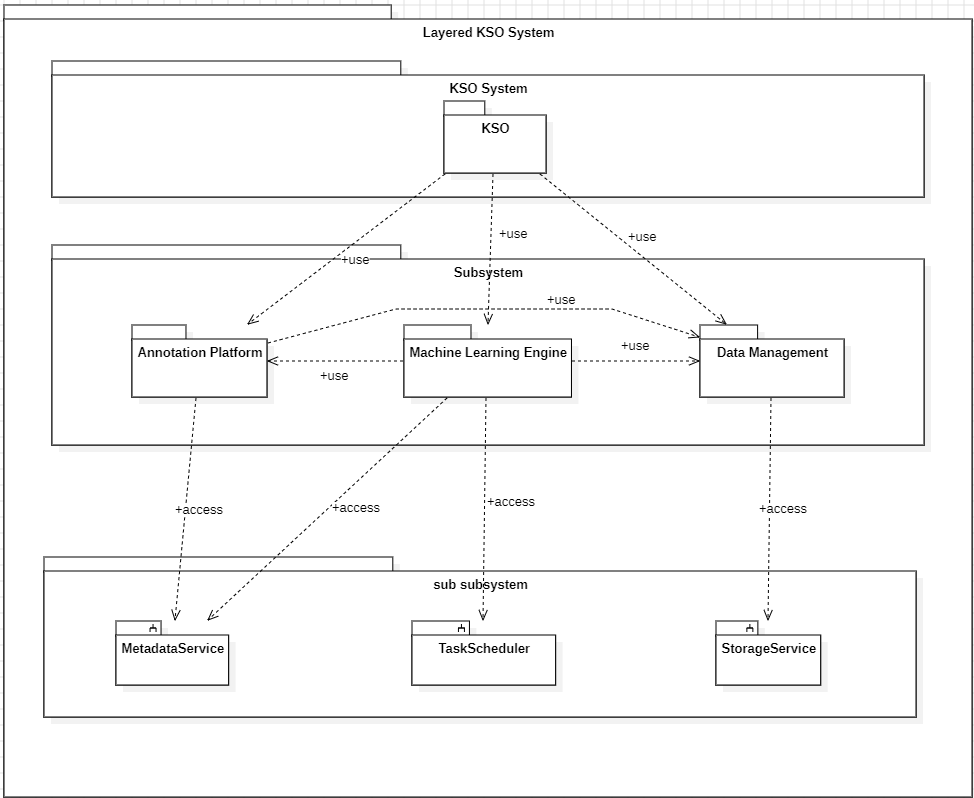
\includegraphics[width=1 \textwidth]{Figures/PackageDiagram.png}
    \caption{Package Diagram \label{Fig:Package Diagram}}
\end{figure}

At \textbf{Level 0}, the top-level package is the \textit{Koster Seafloor Observatory (KSO)} system, which encapsulates all major software components responsible for the storage, annotation, and automated analysis of subsea video data. The system integrates citizen science contributions with machine learning pipelines to support large-scale marine biodiversity monitoring. This layered architecture promotes separation of concerns, scalability, and modular reuse.

At \textbf{Level 1}, the system is divided into three primary subsystems. The \texttt{AnnotationPlatform} provides the web interface and functionality for citizen scientists to annotate video clips. It fetches clip and species metadata to display tasks and enables annotation submissions. The \texttt{MachineLearningEngine} subsystem manages the end-to-end machine learning workflow, including training models based on human annotations and applying those models to unlabeled video clips for automated species detection. It accesses shared services to retrieve input data and uses scheduling support for long-running background jobs. The third subsystem, \texttt{DataManagement}, orchestrates storage operations, including the movement of video files between cold (long-term) and hot (active) storage tiers. It ensures that relevant media are available to both the annotation and machine learning workflows.

At \textbf{Level 2}, three shared sub-subsystems provide core infrastructure services. The \texttt{MetadataService} enables querying and updating structured metadata related to media, species, annotations, and tasks. It is accessed by both the annotation and machine learning subsystems to coordinate consistent data usage. The \texttt{StorageService} is accessed solely by the \texttt{DataManagement} subsystem and provides an abstraction over physical storage systems, handling file retrieval and transfer. The \texttt{TaskScheduler} supports the \texttt{MachineLearningEngine} by managing background tasks such as model training and batch inference runs.

In terms of inter-package dependencies, the \texttt{MachineLearningEngine} retrieves human annotations from the \texttt{AnnotationPlatform} and accesses raw video clips via \texttt{DataManagement} for training and inference. Both these subsystems also interact with the \texttt{MetadataService} for task and species metadata. The \texttt{TaskScheduler} is used solely by the \texttt{MachineLearningEngine} for scheduling asynchronous jobs.

\section{Deployment View}

\subsection{Stakeholders’ Uses of This View}

This deployment view addresses the concerns of the following stakeholders:

\begin{itemize}
  \item \textbf{System Integrators} 
Rely on the deployment view to understand the distribution of software components across hardware environments. They use this view to configure data flow pipelines (e.g., video transfer from field station to cold storage, annotation exchanges with Zooniverse) and ensure volume mounts and network links are correctly established for Docker-based components.

\item \textbf{DevOps and Infrastructure Engineers} 
Use this view to plan infrastructure provisioning and resource allocation. They are responsible for deploying JupyterHub (Cloudina), mounting persistent storage (hot storage), and managing the execution environments on the HPC server. This view helps identify the containers (YOLO training, SQLite access) and their required volumes or access protocols (NFS, SCP, HTTPS).

\item \textbf{Researchers and Data Scientists} 
Understand where and how various notebooks run, where to fetch or store processed data, and how to retrieve annotations. They use this view to know which scripts (e.g., \texttt{train\_models.py}, \texttt{publish\_observations.py}) run in which environments, and how the SQLite database integrates with their workflow.

\item \textbf{Citizen Science Coordinators} 
While not directly managing deployments, they rely on this view to understand the flow of data to and from Zooniverse, ensuring the correct upload and retrieval mechanisms are in place for volunteer contributions.

\item \textbf{Marine Biologists and Analysts} 
Benefit from understanding how raw footage collected in the field is integrated into the analysis pipeline. This view clarifies the relationship between field station outputs (e.g., .mp4, .csv files) and downstream tools used for annotation and ecological evaluation.
\end{itemize}

\subsection{Deployment Diagram}

\begin{figure}[H]
  \centering
  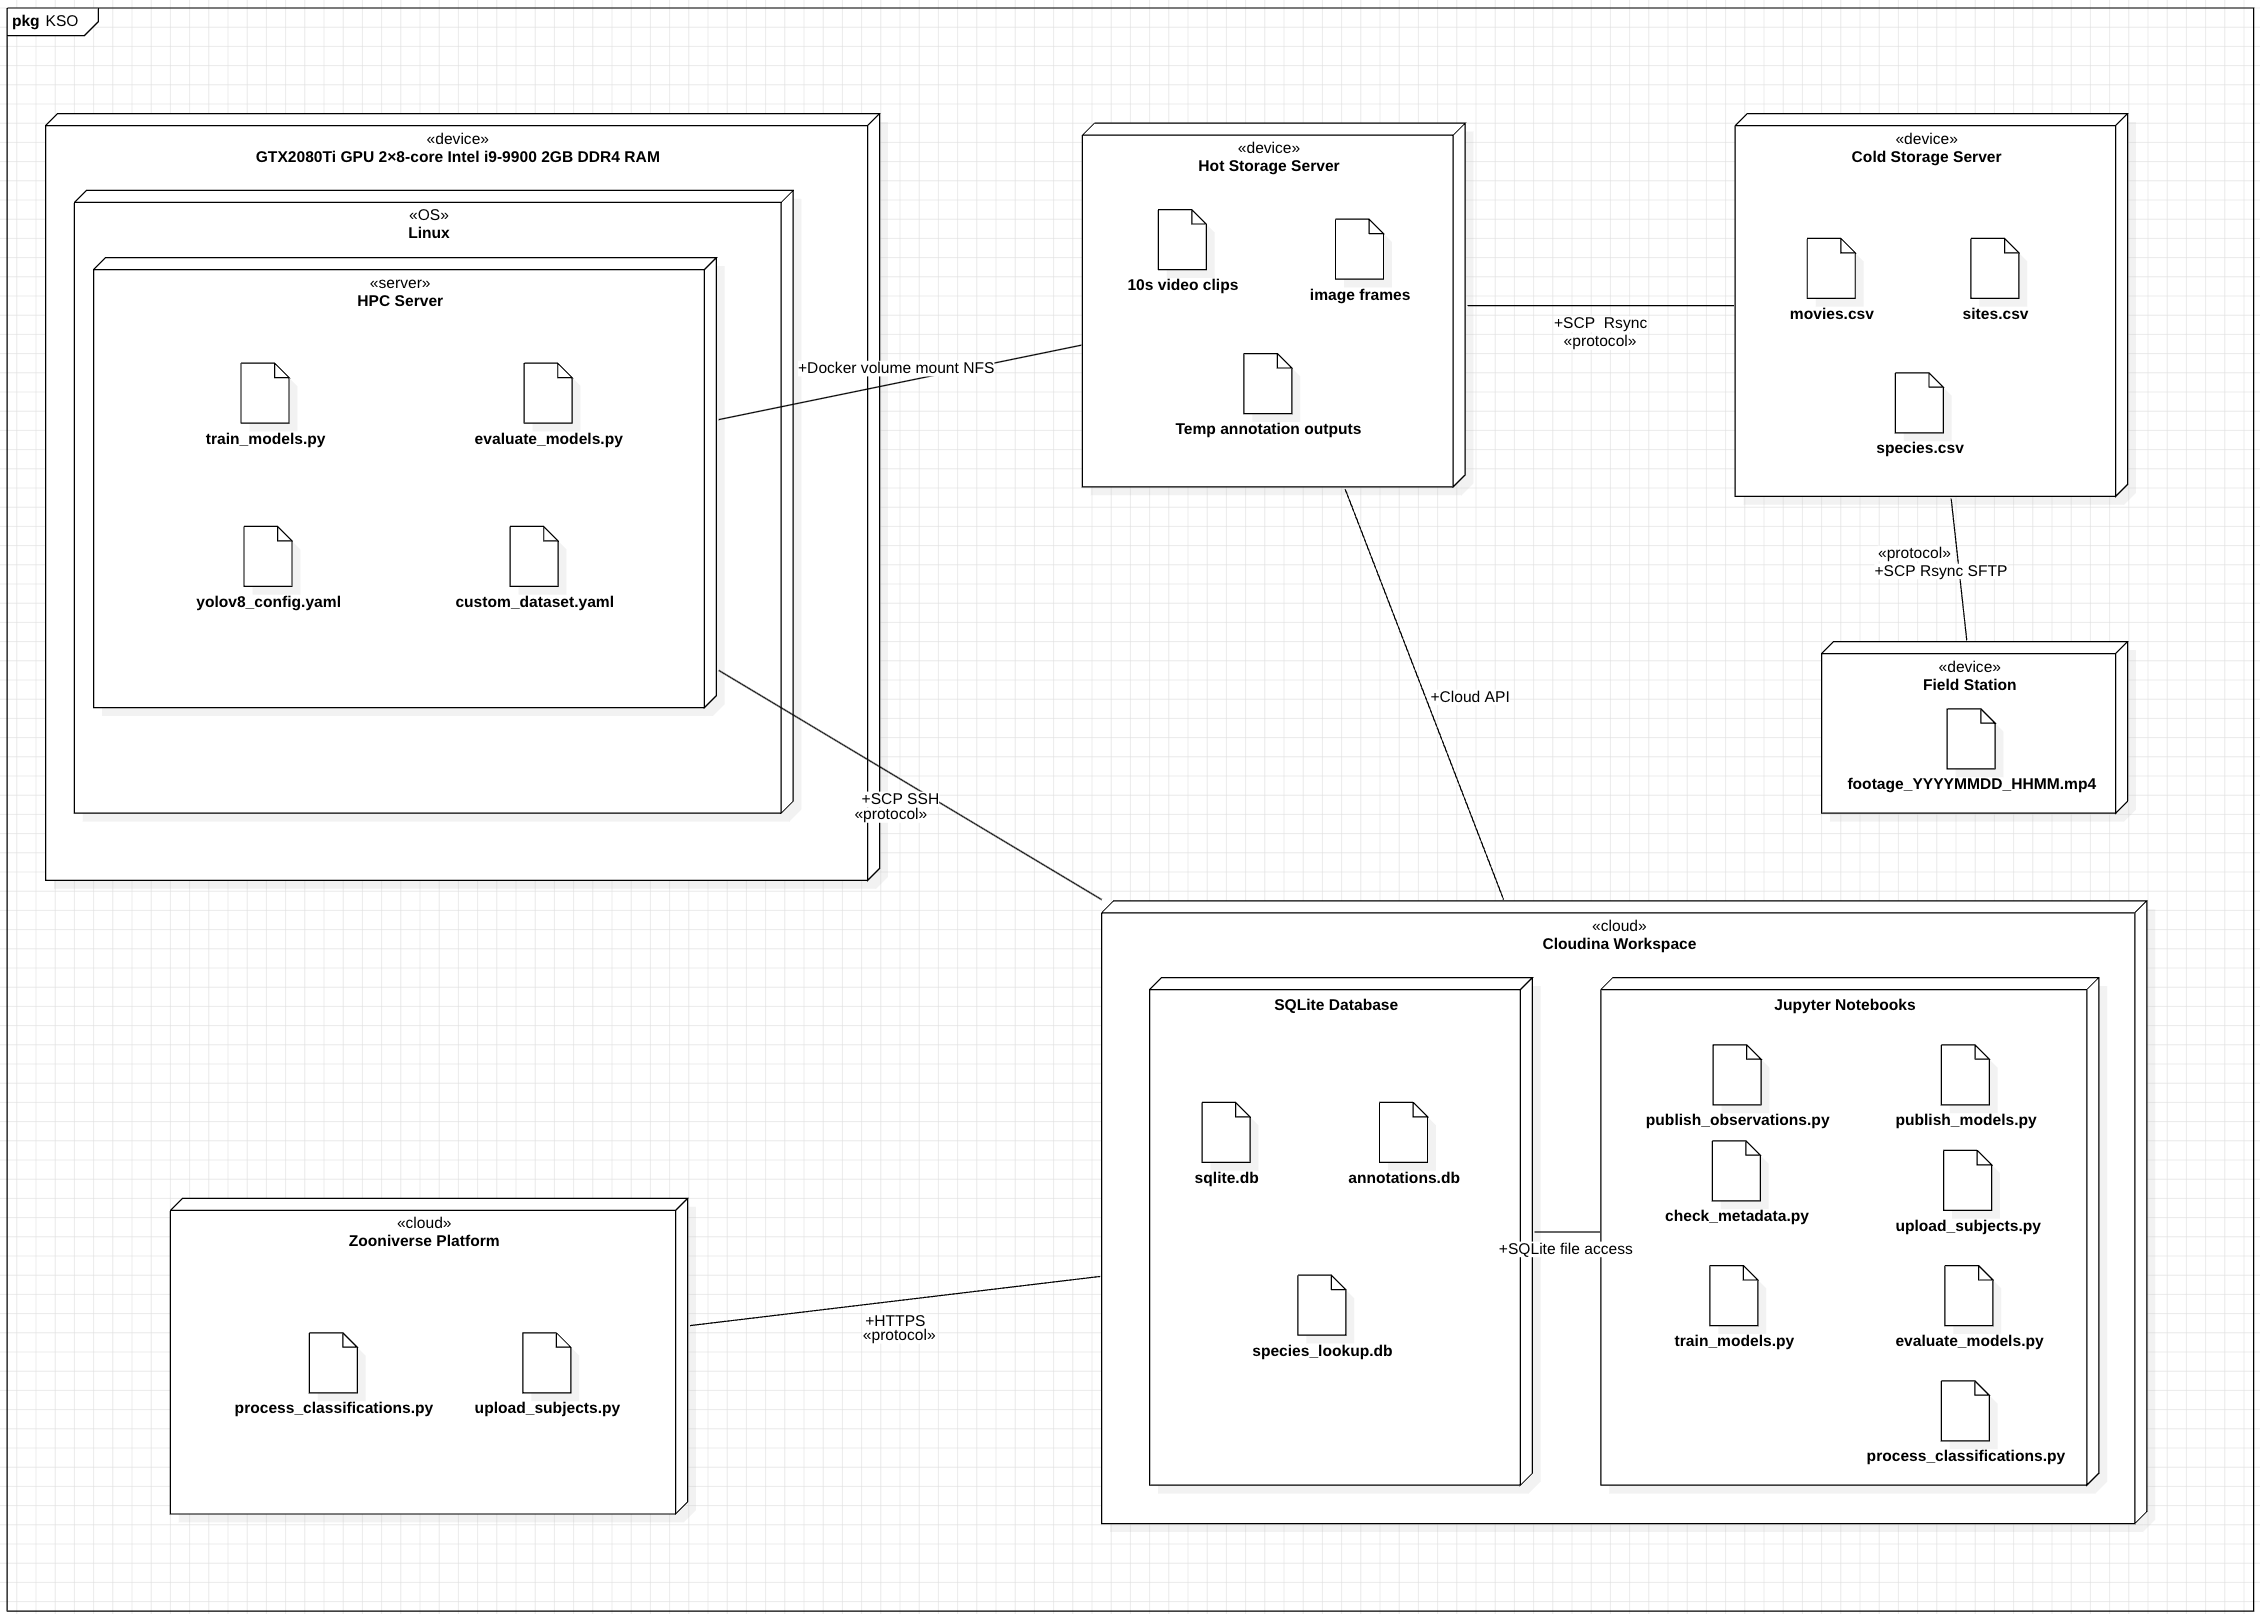
\includegraphics[width=1 \textwidth]{Figures/DeploymentDiagram.png}
  \caption{Deployment Diagram \label{Fig:Deployment Diagram}}
\end{figure}


The Deployment Diagram for the Koster Seafloor Observatory (KSO) illustrates the physical allocation of key software and data components across the system’s infrastructure. It models the environment where system execution occurs, including both physical devices (e.g., Field Station, HPC Server) and virtual/cloud-based services (e.g., Zooniverse, Cloudina).

The field station collects raw footage and contextual metadata, which is transferred to a Cold Storage Server hosted at the University of Gothenburg for archival. A subset of this data is copied to the Hot Storage Server, which acts as short-term, fast-access storage for active analysis and annotation preparation. Jupyter Notebooks are executed in the Cloudina Workspace (a JupyterHub-based environment), which accesses both the video clips and a local SQLite database used to manage metadata, annotations, and export-ready records.

The Zooniverse platform is used by citizen scientists to annotate subsea imagery. Cloudina scripts interact with Zooniverse via HTTPS using the \texttt{panoptes\_client} API to upload frames and fetch classification results. These results are then used to prepare training datasets for machine learning models.

The HPC Server at Chalmers runs a containerized training environment (typically YOLOv5 or YOLOv8) and accesses training data via mounted volumes from the Hot Storage Server. The server does not contain its own persistent database and instead operates statelessly with inputs provided from Cloudina and outputs pushed back to shared storage.

Communication protocols such as rsync, scp, NFS, and RESTful HTTPS APIs are employed to enable data movement and service interaction across nodes. The SQLite database remains local to Cloudina, reinforcing the separation between storage (object-based) and structured metadata access (query-based).

This deployment view ensures modularity, reproducibility, and scalability in processing large-scale underwater ecological data across hybrid research infrastructures.

\newpage
\section{Design Rationale}

\begin{itemize}
  \item \textbf{Functional View}: We partitioned the system into three high-level modules—Data Management, Citizen Science, and Machine Learning—to maximize cohesion within each module while keeping coupling low. This modular structure lets us evolve or scale each capability independently as data volumes grow, at the cost of defining clear inter-module interfaces early on.
  \item \textbf{Information View}: We chose a Darwin Core–compliant SQLite relational schema \cite{anton2021kso} for storing movies, annotations, metadata, and model results. By adhering to a widely-adopted biodiversity data standard, we ensure seamless data sharing and reuse across research infrastructures, accepting moderate query-performance overhead in exchange for interoperability.
  \item \textbf{Development View}: We organized the codebase into a three-level modular hierarchy (Level 0: KSO, Level 1: subsystems like the Zooniverse connector, ML model, and API, Level 2: their internal packages) to enable parallel workstreams for data engineers, ML developers, and front-end teams. This increases upfront architectural complexity but dramatically reduces merge conflicts and integration risk as the project scales.
  \item \textbf{Deployment View}: We deploy each subsystem as a containerized microservice on our HPC cluster—Data Management on CPU nodes, ML inference on GPU nodes, and a lightweight Streamlit front-end—so that compute resources are matched to workload (high-throughput video processing vs. low-latency web UI). This delivers high performance and flexibility at the expense of more sophisticated orchestration and monitoring.
\end{itemize}